\documentclass[11pt,a4paper]{article}

\usepackage[T1]{fontenc}
\usepackage{lmodern}
\usepackage[margin=2.25cm]{geometry}
\usepackage{graphicx}
\usepackage{booktabs}
\usepackage{amsmath,amssymb}
\usepackage{xcolor}
\usepackage{hyperref}
\usepackage{listings}
\usepackage{enumitem}
\usepackage{caption}
\usepackage{subcaption}
\usepackage{array}
\usepackage{multirow}
\usepackage{microtype}

\graphicspath{{../results/pcla_large_scale_constrained_dirichlet_v1/figures/}}

\definecolor{navy}{HTML}{17365D}
\definecolor{blue}{HTML}{2F5597}
\definecolor{lightblue}{HTML}{D9EAF7}
\definecolor{green}{HTML}{548235}
\definecolor{orange}{HTML}{C55A11}
\definecolor{lightgray}{HTML}{F2F2F2}
\definecolor{codegray}{HTML}{444444}

\hypersetup{
  colorlinks=true,
  linkcolor=navy,
  citecolor=green,
  urlcolor=blue,
  pdftitle={PCLA: Client-Specific Component-Level LoRA Allocation for Federated Fine-Tuning}
}

\lstset{
  language=Python,
  basicstyle=\ttfamily\small,
  keywordstyle=\color{blue}\bfseries,
  commentstyle=\color{green},
  stringstyle=\color{orange},
  numbers=left,
  numberstyle=\tiny\color{codegray},
  frame=single,
  backgroundcolor=\color{lightgray},
  breaklines=true,
  showstringspaces=false,
  tabsize=2
}

\newcommand{\method}{\textsc{PCLA-Component}}
\newcommand{\fedhello}{\textsc{FedHeLLo-Controlled}}
\newcommand{\fedlora}{\textsc{FedLoRA}}
\newcommand{\randomcomp}{\textsc{Random-Component}}
\newcommand{\pp}{\,pp}

\title{\vspace{-1.2cm}
  \textbf{PCLA: Client-Specific Component-Level LoRA Allocation}\\
  \large A Cost-Constrained Method for Communication-Efficient Federated Fine-Tuning
}
\author{Final-Year Project Technical Report\\
  \small Student name and student ID to be inserted}
\date{27 July 2026}

\begin{document}
\maketitle

\begin{abstract}
This report presents the current design, implementation, and large-scale
evaluation of PCLA, our method for resource-aware federated fine-tuning with
Low-Rank Adaptation (LoRA). The current implementation instantiates PCLA at the
level of aligned LoRA rank components: each participating client estimates
client-specific marginal utility for individual components, selects components
under a hard resource budget, alternates the trainable LoRA factor, and
aggregates each component only from clients that actually updated it. On a
20-client SST-2/BERT-base experiment with 30 communication rounds and three
random seeds, PCLA obtains $87.02\%\pm2.57\%$ final accuracy. It is below full
FedLoRA by $2.42$ percentage points and below a controlled FedHeLLo-style
baseline by $1.39$ percentage points, but reduces estimated communication by
$84.40\%$ and $74.68\%$, respectively. Under an exactly matched component
budget, PCLA improves final accuracy over random component allocation by
$8.03$ percentage points. Therefore, the evidence supports an
\emph{accuracy--efficiency trade-off and effective importance-based component
selection}; it does not yet support a claim of superior accuracy over
FedLoRA or FedHeLLo.
\end{abstract}

\section{Research objective and contribution boundary}

Federated fine-tuning must accommodate clients with different computation and
communication capabilities. Training the same LoRA structure on every client
is simple, but it ignores resource heterogeneity. Existing heterogeneous LoRA
methods already vary ranks or trainable layers across clients
\cite{hetlora,flora,fedhello}. Our project therefore does not claim that
combining resource information with LoRA importance is new by itself.

The narrower research question is:
\begin{quote}
\emph{Can a federated system use client-specific, component-level marginal
utility to allocate a fixed LoRA budget more effectively than a matched random
allocation, while preserving stable aggregation under heterogeneous and
partially overlapping updates?}
\end{quote}

The current contribution is a complete mechanism containing:
\begin{enumerate}[leftmargin=1.6em]
  \item aligned rank-component selection rather than whole-layer selection;
  \item persistent, client-specific importance state with temporal smoothing,
  exploration and freshness;
  \item hard per-client capacity constraints;
  \item alternating optimization of the two LoRA factors;
  \item contributor-only aggregation for partially overlapping updates; and
  \item a corrected, auditable non-IID partition and matched-budget evaluation.
\end{enumerate}

The project name PCLA originally denotes \emph{Personalized Cost-aware LoRA
Allocation}. In the present implementation, ``personalized'' refers to
client-specific allocation state, not a separate final prediction model for
each client. ``Cost-aware'' is currently implemented mainly as a hard capacity
and communication budget; it is not yet a learned continuous cost model.

\section{Background and related work}

\subsection{Federated averaging and LoRA}

Federated Averaging (FedAvg) trains local models on decentralized data and
forms a sample-weighted average at the server \cite{fedavg}. LoRA freezes the
pre-trained weight matrix and learns a low-rank update
\cite{lora}:
\begin{equation}
  W' = W + \Delta W,\qquad
  \Delta W = \frac{\alpha}{r}BA,
  \label{eq:lora}
\end{equation}
where $A\in\mathbb{R}^{r\times d_{\mathrm{in}}}$,
$B\in\mathbb{R}^{d_{\mathrm{out}}\times r}$, rank $r$ is small, and the
pre-trained $W$ remains frozen. This reduces trainable parameters, although a
federated system must still decide which LoRA parameters each heterogeneous
client can train.

\subsection{Closest heterogeneous LoRA methods}

\textsc{HetLoRA} studies heterogeneous LoRA ranks across clients
\cite{hetlora}. \textsc{FLoRA} also addresses heterogeneous low-rank
adaptations and their aggregation \cite{flora}. \textsc{FedHeLLo} allocates
trainable LoRA layers according to client resource capability and layer
importance \cite{fedhello}. Sparse LoRA work such as \textsc{SoRA} shows that
rank components can be pruned or sparsified rather than treating the rank as an
indivisible unit \cite{sora}. \textsc{FedHL} further highlights that naive
aggregation under heterogeneous low-rank updates can be biased
\cite{fedhl}.

PCLA is closest to FedHeLLo in its use of resource capability and importance.
The operational difference in this project is granularity and state:
FedHeLLo-style allocation chooses important \emph{layers}, whereas PCLA scores
aligned \emph{rank components} for each client and retains client-specific
history across partial participation. This is a focused extension to be tested,
not a claim that all ingredients are individually novel.

\section{Problem formulation}

Let $K$ be the number of clients and $\mathcal{S}_t$ the subset selected at
round $t$. Client $k$ has local dataset $\mathcal{D}_k$ with
$n_k=|\mathcal{D}_k|$ and a resource capacity $q_k$. In the reported
experiment, $q_k\in\{6,9,12\}$ denotes an active-layer-equivalent budget. Since
each active layer has $m=8$ selected rank components, client $k$ can update at
most
\begin{equation}
  C_k=q_km
\end{equation}
component positions in a sparse round.

For LoRA rank $r$, Equation~\ref{eq:lora} can be decomposed as
\begin{equation}
  BA = \sum_{j=1}^{r} b_j a_j^\top ,
  \label{eq:components}
\end{equation}
where $b_j$ is column $j$ of $B$ and $a_j^\top$ is row $j$ of $A$. A component
identifier is aligned by transformer layer, projection type
(\texttt{query}/\texttt{value}), and rank index $j$. PCLA seeks a binary mask
$z_{k,c,t}\in\{0,1\}$ that maximizes estimated client-specific utility under
the capacity constraint
\begin{equation}
  \max_{\mathbf z_{k,t}}\sum_c s_{k,c,t}z_{k,c,t}
  \quad\text{subject to}\quad
  \sum_c z_{k,c,t}\le C_k,
  \label{eq:allocation}
\end{equation}
with an additional layer-coverage rule described below.

\section{PCLA algorithm design}

\subsection{First-order component importance}

PCLA estimates the marginal utility of component $j$ from one local batch.
When $B$ is trainable, the score for one projection is
\begin{equation}
  I^{(B)}_{k,j}=\left\|\nabla_{b_j}\mathcal{L}_k\right\|_2
                    \left\|a_j\right\|_2 .
  \label{eq:importance-b}
\end{equation}
When $A$ is trainable, it uses
\begin{equation}
  I^{(A)}_{k,j}=\left\|b_j\right\|_2
                    \left\|\nabla_{a_j}\mathcal{L}_k\right\|_2 .
  \label{eq:importance-a}
\end{equation}
Scores from the query and value projections are added for the aligned
layer--rank component. These expressions approximate the first-order effect of
changing one low-rank outer product while accounting for the magnitude of its
frozen counterpart.

\subsection{Persistent client-specific score}

Raw importance is normalized within a client and smoothed using an exponential
moving average:
\begin{equation}
  \bar{\mathbf I}_{k,t} =
  \operatorname{Norm}\!\left(
  \rho\bar{\mathbf I}_{k,t^-}+(1-\rho)\operatorname{Norm}(\mathbf I_{k,t})
  \right),
  \qquad \rho=0.8 .
\end{equation}
The allocation score is
\begin{equation}
 s_{k,c,t} =
 \operatorname{Std}(\bar I_{k,c,t})
 +\beta\sqrt{\frac{\log(t+1)}{N_{k,c,t}+1}}
 +\gamma\min\!\left(\frac{A_{k,c,t}}{\max(t-1,1)},1\right)
 +\delta\,\mathbb{1}[c\in M_{k,t^-}],
 \label{eq:score}
\end{equation}
where $N_{k,c,t}$ is the number of prior selections and $A_{k,c,t}$ is the
age of the stored score. The main experiment uses $\beta=0.5$,
$\gamma=0.05$, and $\delta=0$. The exploration term prevents permanent early
lock-in, while freshness gives modest preference to stale components.

Importance is initialized the first time a client participates and refreshed
when at least three rounds have elapsed since that client's last refresh. The
state survives rounds in which the client is not selected.

\subsection{Capacity-constrained hierarchical selection}

Directly taking the global top $C_k$ components can concentrate all updates in
a few layers. PCLA therefore uses a two-stage rule:
\begin{enumerate}[leftmargin=1.6em]
  \item For every transformer layer, calculate the mean of its top $m$
  component scores.
  \item Select the top $q_k$ layers.
  \item Allocate at least one component to each selected layer.
  \item Fill the remaining $q_km-q_k$ positions using the highest component
  scores within those selected layers.
\end{enumerate}
This preserves layer coverage while allowing the component distribution within
the chosen layers to adapt to each client.

\subsection{Alternating LoRA-factor optimization}

If both factors are updated simultaneously, a component mask does not cleanly
isolate the marginal contribution of one outer-product factor. PCLA alternates:
odd sparse rounds train $B$ while freezing $A$, and even sparse rounds train
$A$ while freezing $B$. Only selected component rows or columns receive
gradients. The classifier head is trained by all selected clients.

\subsection{Contributor-only aggregation}

For component $c$, let
$\mathcal{C}_{c,t}=\{k\in\mathcal{S}_t:z_{k,c,t}=1\}$ be its contributors.
The server aggregates only those clients:
\begin{equation}
  \theta_{c,t+1} =
  \begin{cases}
  \displaystyle
  \frac{\sum_{k\in\mathcal{C}_{c,t}}n_k\theta_{k,c,t}}
       {\sum_{k\in\mathcal{C}_{c,t}}n_k},
       & \mathcal{C}_{c,t}\ne\varnothing,\\[1.2em]
  \theta_{c,t}, & \mathcal{C}_{c,t}=\varnothing.
  \end{cases}
  \label{eq:aggregation}
\end{equation}
Thus an unchanged value from a non-contributing client cannot dilute an actual
update. The classifier is sample-weight averaged over all selected clients.

\subsection{End-to-end procedure}

\begin{lstlisting}[caption={High-level PCLA server procedure.},label={lst:pcla}]
for round_id in range(1, num_rounds + 1):
    selected_clients = sample_clients(round_id)
    factor = component_round_schedule(round_id)  # B, A, B, A, ...

    for client in selected_clients:
        if should_refresh_client_importance(client, round_id):
            score = estimate_component_importance(
                global_model, client, factor, one_batch=True)
            client_state[client].update_ema(score)

        mask = select_component_allocation(
            client_state[client], capacity[client],
            components_per_layer=8)
        local_update = train_client_components(
            global_model, client, mask, train_factor=factor)
        uploads.append(local_update)

    global_model = aggregate_component_models(
        global_model, uploads, contributor_only=True)
\end{lstlisting}

\section{Corrected non-IID data partition}

An earlier label-skew procedure independently rounded the positive count for
each client after a Dirichlet draw. This could move the aggregate class prior
away from the source dataset and create an unintended easier or harder test
condition. Those earlier results are retained only as diagnostic runs.

The formal experiment uses a constrained construction. It first draws
heterogeneous client label odds, then applies one common shift in log-odds so
that the expected counts satisfy both:
\begin{enumerate}[leftmargin=1.6em]
  \item the fixed row sum of 512 samples for every client; and
  \item the fixed global column sum of 5,712 positive examples out of 10,240.
\end{enumerate}
Integer counts are assigned by largest-remainder rounding, and examples are
sampled without replacement. This preserves substantial client-level label
skew without altering the global SST-2 class prior.

\section{Implementation map}

The implementation is contained in
\texttt{pcla\_experiments/src/fedhello\_sst2.py}. Table~\ref{tab:impl} maps the
algorithmic ideas to the executable functions.

\begin{table}[htbp]
\centering
\caption{Algorithm-to-code mapping.}
\label{tab:impl}
\small
\begin{tabular}{>{\raggedright\arraybackslash}p{0.27\linewidth}
                >{\raggedright\arraybackslash}p{0.32\linewidth}
                >{\raggedright\arraybackslash}p{0.33\linewidth}}
\toprule
Component & Main implementation & Responsibility\\
\midrule
Masked LoRA forward pass
& \texttt{LoRALinear}
& Registers component masks and applies them to aligned rank dimensions.\\
Factor alternation
& \texttt{component\_round\_schedule}
& Chooses the trainable $A$ or $B$ factor for each sparse round.\\
Refresh policy
& \texttt{should\_refresh\_client\_importance}
& Initializes and periodically refreshes per-client state.\\
Budgeted selection
& \texttt{select\_component\_allocation}
& Scores layers and components, then enforces capacity and coverage.\\
Corrected non-IID split
& \texttt{constrained\_dirichlet\_positive\_counts}
& Preserves client sample totals and the global class total.\\
Mask application
& \texttt{set\_component\_masks}
& Activates only the selected aligned component indices.\\
Importance estimation
& \texttt{estimate\_component\_importance}
& Computes Equations~\ref{eq:importance-b}--\ref{eq:importance-a}.\\
Sparse local training
& \texttt{train\_client\_components}
& Trains the selected components and chosen LoRA factor.\\
Stable aggregation
& \texttt{aggregate\_component\_models}
& Implements contributor-only aggregation in Equation~\ref{eq:aggregation}.\\
\bottomrule
\end{tabular}
\end{table}

The experiment configuration is
\texttt{configs/pcla\_large\_scale\_constrained\_dirichlet.json}. The output
directory is
\texttt{results/pcla\_large\_scale\_constrained\_dirichlet\_v1}.

\section{Experimental methodology}

\subsection{Protocol}

\begin{table}[htbp]
\centering
\caption{Formal large-scale experiment protocol.}
\label{tab:protocol}
\small
\begin{tabular}{ll}
\toprule
Item & Setting\\
\midrule
Task / backbone & SST-2 / BERT-base-uncased\\
Federated scale & 20 total clients, 10 selected per round\\
Training horizon & 30 communication rounds\\
Client data & 512 training examples per client\\
Non-IID partition & Constrained Dirichlet, $\alpha=0.3$\\
Random seeds & 7, 13, 21\\
Resource groups & $6:3:1$ clients with capacities 6, 9, 12 layers\\
LoRA & Rank 16, scaling 16, dropout 0.1\\
Target modules & BERT query and value projections\\
PCLA component budget & 8 components per active-layer-equivalent\\
Importance refresh & Interval 3, EMA 0.8, one batch per client\\
Exploration / freshness & $\beta=0.5$, $\gamma=0.05$\\
\bottomrule
\end{tabular}
\end{table}

\subsection{Compared methods}

\begin{description}[style=nextline,leftmargin=0em]
  \item[\fedlora] All clients train all LoRA parameters. This is the
  highest-capacity accuracy reference.
  \item[\fedhello] A controlled FedHeLLo-style mechanism that selects whole
  LoRA layers using resource capacity and layer importance. It is not claimed
  to be an exact numerical reproduction of every setting in the FedHeLLo paper.
  \item[\randomcomp] Selects aligned rank components randomly under exactly the
  same client participation, capacity, parameter and communication budgets as
  PCLA.
  \item[\method] Uses the client-specific importance and allocation mechanism
  in Section~4 under the matched component budget.
\end{description}

\subsection{Fairness and audit checks}

The experimental validator passed 25 unit tests. For each seed, the run
produced 120 method-level metrics, 1,200 allocation records and 57,708
importance records. Across all 900 paired client-round observations,
\method{} and \randomcomp{} have identical selected clients, capacity,
trainable-parameter count, communication estimate and trainable factor.
Therefore, their difference isolates the allocation policy rather than budget
or participation.

\subsection{Efficiency metrics}

Estimated client traffic is
\begin{equation}
  \operatorname{MB}_{k,t} =
  \frac{2\times 4\times P_{k,t}}{2^{20}},
  \label{eq:comm}
\end{equation}
where $P_{k,t}$ is the number of selected trainable parameters, 4 bytes denotes
FP32, and the factor 2 represents download plus upload.

The reported time is a controlled simulation:
\begin{equation}
 T_t =
 \max_{k\in\mathcal{S}_t}
 \left(
 T^{\mathrm{measured}}_{k,t}f^{\mathrm{compute}}_k+
 1.5\,\operatorname{MB}_{k,t}f^{\mathrm{comm}}_k
 \right)
 +T^{\mathrm{importance}}_t .
 \label{eq:time}
\end{equation}
It models synchronous stragglers and heterogeneous compute/communication
factors. Consequently, the report calls it \emph{simulated time}, not measured
wall-clock network time.

\section{Results}

\subsection{Aggregate results across three seeds}

\begin{table}[htbp]
\centering
\caption{Large-scale results. Accuracy is mean $\pm$ standard deviation over
three seeds. Time is simulated according to Equation~\ref{eq:time}.}
\label{tab:results}
\small
\setlength{\tabcolsep}{5pt}
\begin{tabular}{lrrrrr}
\toprule
Method & Final acc. & Late-5 acc. & Round avg. & Time (s) & Comm. (MB)\\
\midrule
\fedlora
& $\mathbf{89.43\pm0.38}$ & $\mathbf{87.98}$ & $\mathbf{81.37}$
& 314.00 & 1353.52\\
\fedhello
& $88.41\pm1.61$ & $86.67$ & $80.30$
& 183.89 & 834.15\\
\method
& $87.02\pm2.57$ & $83.65$ & $78.00$
& 100.19 & \textbf{211.18}\\
\randomcomp
& $78.99\pm6.43$ & $73.70$ & $70.37$
& \textbf{73.15} & \textbf{211.18}\\
\bottomrule
\end{tabular}
\end{table}

PCLA's importance estimation takes 25.61 seconds, or 25.56\% of its simulated
time. This explains why it is slower than the matched random allocator despite
identical communication and trainable-parameter budgets.

\subsection{Matched-budget causal comparison}

Relative to \randomcomp{}, PCLA improves:
\begin{align*}
  \text{final accuracy} &: +8.03\pp,\\
  \text{late-5-round accuracy} &: +9.95\pp,\\
  \text{round-average accuracy} &: +7.62\pp.
\end{align*}
The final-accuracy improvement is positive for every seed:
$+4.71\pp$, $+6.70\pp$, and $+12.68\pp$ for seeds 7, 13 and 21,
respectively. This is the cleanest evidence that the learned allocation is
useful.

\subsection{Accuracy--efficiency trade-off}

Against \fedhello{}, PCLA gives up $1.39\pp$ final accuracy while reducing
communication by 74.68\% and simulated time by 45.52\%. Against full
\fedlora{}, it gives up $2.42\pp$ while reducing communication by 84.40\% and
simulated time by 68.09\%. These are substantial estimated efficiency gains,
but they should be presented together with the accuracy loss.

\begin{figure}[htbp]
\centering
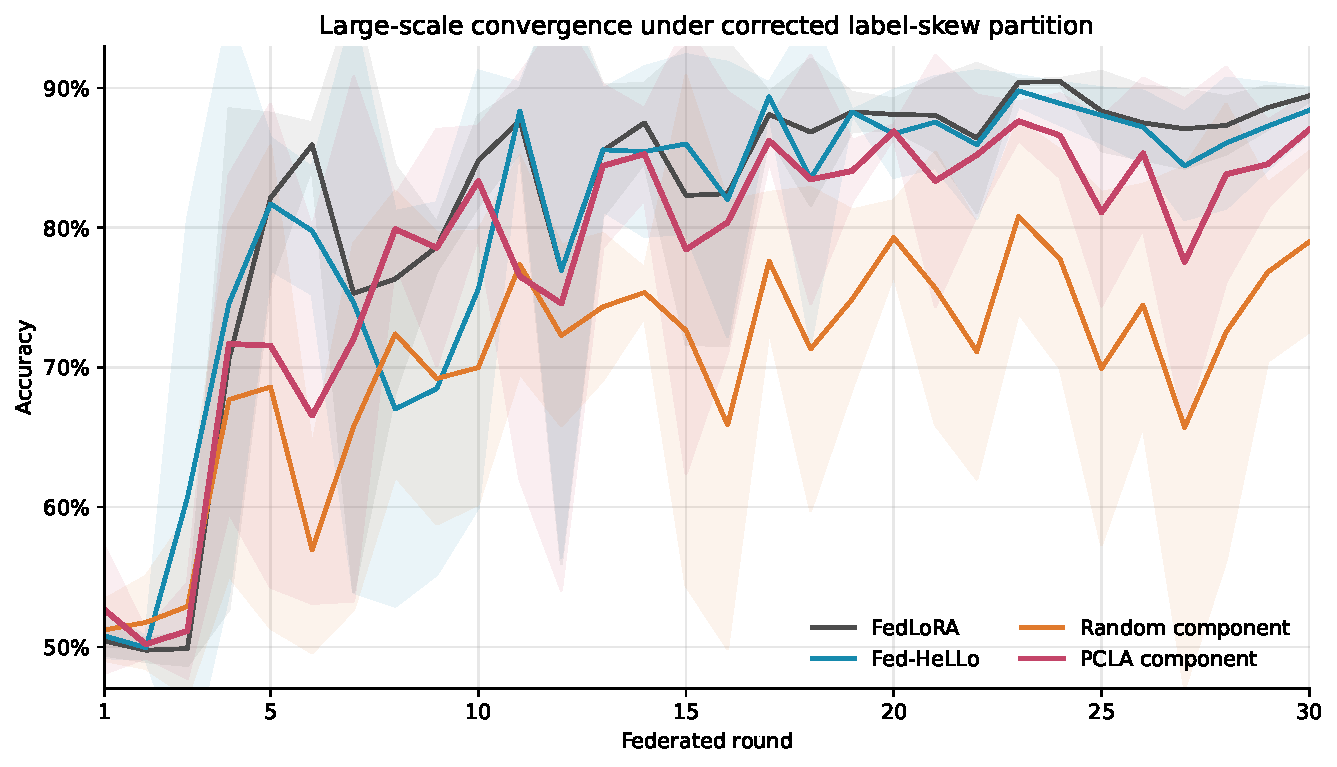
\includegraphics[width=0.96\linewidth]{large_scale_convergence.pdf}
\caption{Mean validation accuracy over 30 rounds; the shaded region represents
variation across three seeds. PCLA consistently exceeds the exactly matched
random component allocator.}
\label{fig:convergence}
\end{figure}

\begin{figure}[htbp]
\centering
\begin{subfigure}[t]{0.48\linewidth}
  \centering
  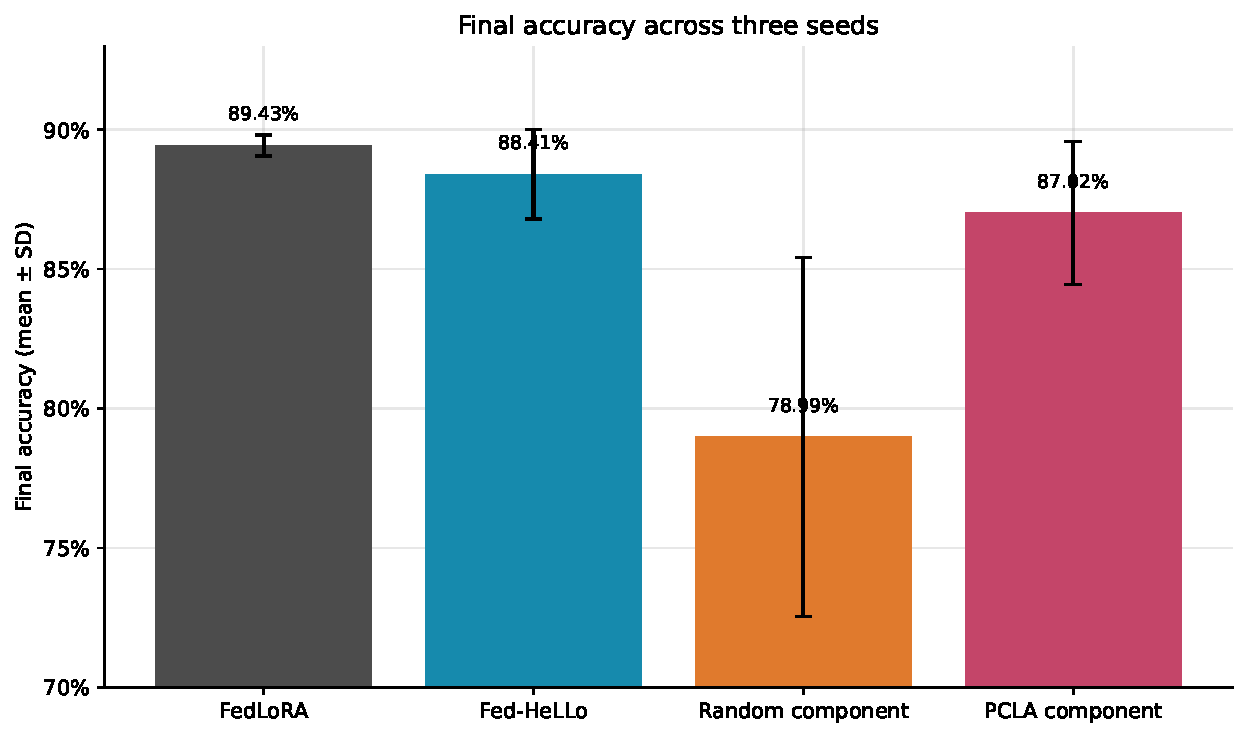
\includegraphics[width=\linewidth]{large_scale_final_accuracy.pdf}
  \caption{Final accuracy.}
\end{subfigure}
\hfill
\begin{subfigure}[t]{0.48\linewidth}
  \centering
  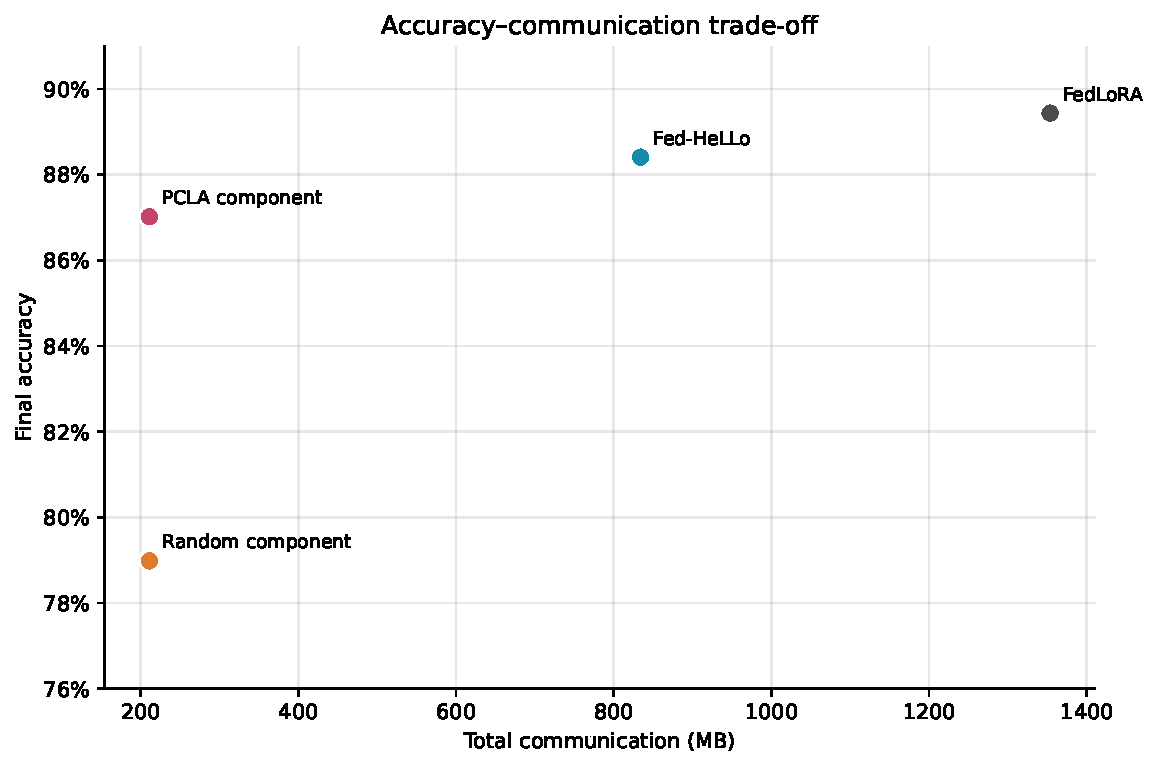
\includegraphics[width=\linewidth]{large_scale_accuracy_communication.pdf}
  \caption{Accuracy versus communication.}
\end{subfigure}
\caption{Final performance and the accuracy--communication operating points.}
\label{fig:tradeoff}
\end{figure}

\section{What the experiment establishes}

\subsection{Claims supported by the current evidence}

\begin{enumerate}[leftmargin=1.6em]
  \item Under identical client participation and component budgets,
  importance-based PCLA allocation is materially better than random allocation.
  \item PCLA reaches a competitive SST-2 accuracy while using substantially
  lower protocol-level communication than the layer-level and full-LoRA
  references.
  \item Contributor-only aggregation and persistent per-client state execute
  correctly under heterogeneous, partially overlapping allocations.
  \item The formal result is based on a corrected partition that preserves the
  global class prior and on three complete seeds.
\end{enumerate}

\subsection{Claims not supported yet}

\begin{enumerate}[leftmargin=1.6em]
  \item PCLA is not more accurate than FedLoRA or the controlled FedHeLLo-style
  baseline in this experiment.
  \item The experiment does not demonstrate generalization beyond one task,
  one backbone and one heterogeneity level.
  \item The time results are not measurements from real federated devices or a
  real communication network.
  \item The controlled FedHeLLo result is a mechanism comparison, not an exact
  reproduction of the paper's complete CIFAR-100 protocol.
  \item The experiment does not yet isolate every PCLA design choice through
  ablation.
\end{enumerate}

\section{Limitations and next experiments}

\paragraph{Dense computation behind a sparse mask.}
The current PyTorch implementation masks rank components but still executes
dense rank-16 operations in selected layers. Equation~\ref{eq:comm} represents
a sparse communication protocol assuming the frozen backbone and frozen LoRA
factor are cached client-side; it is not evidence of an implemented sparse GPU
kernel or real socket traffic.

\paragraph{Importance overhead.}
Importance estimation consumes 25.56\% of PCLA's simulated time. The highest
priority efficiency experiment is therefore an adaptive refresh policy:
refresh only when the client's allocation or importance distribution changes
enough, and compare it with intervals 1, 3 and 5.

\paragraph{Ablation requirements.}
The next defensible ablations are: no EMA, no exploration, no freshness,
global rather than client-specific importance, no layer-coverage constraint,
and naive aggregation rather than contributor-only aggregation. These identify
which parts produce the matched-random gain.

\paragraph{External validity.}
The result should be repeated on at least one more task or dataset and at
multiple Dirichlet values (for example $\alpha\in\{0.1,0.3,1.0\}$). A formal
FedHeLLo reproduction using its official CIFAR-100 configuration should precede
claims about outperforming that method.

\paragraph{Statistical strength.}
Three seeds are acceptable for a project-stage comparison but remain limited.
Five seeds and paired significance or confidence intervals would make the
matched-budget conclusion stronger.

\section{Presentation-ready conclusion}

The accurate summary for a supervisor presentation is:
\begin{quote}
We developed a client-specific, component-level LoRA allocation method for
heterogeneous federated fine-tuning. PCLA estimates the marginal utility of
aligned LoRA rank components for each participating client, selects them under
a fixed capacity budget, and aggregates only genuine contributors. In a
20-client, 30-round SST-2 experiment, PCLA achieved 87.02\% final accuracy. It
did not beat full FedLoRA or the controlled FedHeLLo-style baseline in absolute
accuracy, but used 84.40\% and 74.68\% less estimated communication,
respectively. Most importantly, it beat a precisely budget-matched random
allocator by 8.03 percentage points, showing that the learned component
allocation---rather than extra parameters or favorable participation---creates
real value.
\end{quote}

\section{Reproducibility}

From the \texttt{pcla\_experiments} directory, the formal suite and audit are
run with:
\begin{lstlisting}[language=bash,numbers=none]
python scripts/run_pcla_large_scale.py \
  --config configs/pcla_large_scale_constrained_dirichlet.json

python scripts/validate_pcla_large_scale.py \
  --result-dir results/pcla_large_scale_constrained_dirichlet_v1
\end{lstlisting}
The exact script names should be checked against the repository entry points
before copying these commands to a new machine; the configuration and result
directory above are the authoritative experiment identifiers.

\begin{thebibliography}{9}

\bibitem{fedavg}
B. McMahan, E. Moore, D. Ramage, S. Hampson, and B. Ag\"uera y Arcas,
``Communication-Efficient Learning of Deep Networks from Decentralized Data,''
\emph{Proceedings of AISTATS}, PMLR 54, 2017.
\url{https://proceedings.mlr.press/v54/mcmahan17a.html}

\bibitem{lora}
E. J. Hu, Y. Shen, P. Wallis, Z. Allen-Zhu, Y. Li, S. Wang, L. Wang, and
W. Chen, ``LoRA: Low-Rank Adaptation of Large Language Models,'' 2021.
\url{https://arxiv.org/abs/2106.09685}

\bibitem{hetlora}
Y. J. Cho, L. Liu, Z. Xu, A. Fahrezi, and G. Joshi,
``Heterogeneous LoRA for Federated Fine-tuning of On-Device Foundation
Models,'' 2024.
\url{https://arxiv.org/abs/2401.06432}

\bibitem{flora}
Z. Wang, Z. Shen, Y. He, G. Sun, H. Wang, L. Lyu, and A. Li,
``FLoRA: Federated Fine-Tuning Large Language Models with Heterogeneous
Low-Rank Adaptations,'' 2024.
\url{https://arxiv.org/abs/2409.05976}

\bibitem{fedhello}
Z. Zhang, P. Liu, J. Xu, and R. Hu,
``Fed-HeLLo: Efficient Federated Foundation Model Fine-Tuning with
Heterogeneous LoRA Allocation,'' 2025.
\url{https://arxiv.org/abs/2506.12213}

\bibitem{sora}
N. Ding, X. Lv, Q. Wang, Y. Chen, B. Zhou, Z. Liu, and M. Sun,
``Sparse Low-rank Adaptation of Pre-trained Language Models,'' 2023.
\url{https://arxiv.org/abs/2311.11696}

\bibitem{fedhl}
Z. Peng, J. Zeng, B. Li, G. Li, S. Chen, and T. Wang,
``FedHL: Federated Learning for Heterogeneous Low-Rank Adaptation via Unbiased
Aggregation,'' 2025.
\url{https://arxiv.org/abs/2505.18494}

\end{thebibliography}

\end{document}
